\documentclass[a4paper,12pt]{report}
\addtolength{\topmargin}{-0.8in}
\setlength\textheight{248mm}
\setlength\textwidth{165mm}
\setlength\oddsidemargin{-2mm}
\setlength\evensidemargin{-2mm}
\usepackage[english]{babel}
\usepackage[a-2u]{pdfx}
\usepackage{graphicx}
\usepackage{caption}
\usepackage{lmodern,textcomp}
\usepackage[T1]{fontenc}
\usepackage{fancyhdr}
\usepackage{xcolor,colortbl}
\usepackage{graphicx}
\usepackage{amssymb}
\usepackage{pgfplots}
\usepackage{multicol}
\usepackage{ulem}
\usepackage{color}
\usepackage{amsmath, amsthm, amssymb}
\usepackage{setspace}
\usepackage{listings}
\usepackage{cancel}
\usepackage{marvosym}
\usepackage{multicol}
\usepackage{fancyvrb}

\makeatletter
\newcommand*{\rom}[1]{\expandafter\@slowromancap\romannumeral #1@}
\makeatother

\definecolor{dkgreen}{rgb}{0,0.6,0}
\definecolor{gray}{rgb}{0.5,0.5,0.5}
\definecolor{mauve}{rgb}{0.58,0,0.82}
\graphicspath{ {../images/} }
\def\columnseprulecolor{\color{black}}
\setlength{\columnseprule}{0.3pt}
\def\title{User documentation}
\def\author{Adam Beneš}
\setlength{\parindent}{0pt}
\def\doubleunderline#1{\underline{\underline{#1}}}\makeatletter
\def\@makechapterhead#1{
	{\parindent \z@ \raggedright \normalfont
		\huge\bfseries \thechapter. #1
		\par\nobreak
		\vskip 20\p@
}}
\def\@makeschapterhead#1{
	{\parindent \z@ \raggedright \normalfont
		\huge\bfseries #1
		\par\nobreak
		\vskip 20\p@
}}
\makeatother

\renewcommand{\chaptermark}[1]{%
	\markboth{#1}{}}

\fancypagestyle{toc}{
	\fancyhf{}
	\renewcommand{\headrulewidth}{0.4pt}
	\renewcommand{\footrulewidth}{0.4pt}
	\fancyhead[C]{}
	\fancyhead[L]{\textbf{\title}}
	\fancyfoot[L]{\author}
	\fancyfoot[C]{}
	\fancyfoot[R]{\thepage}
}

\fancypagestyle{plain}{
	\fancyhf{}
	\renewcommand{\headrulewidth}{0.4pt}
	\renewcommand{\footrulewidth}{0.4pt}
	\fancyhead[C]{}
	\fancyhead[L]{\textbf{\title\ -- \thechapter. \leftmark}}
	\fancyfoot[L]{\author}
	\fancyfoot[C]{}
	\fancyfoot[R]{\thepage}
}


\definecolor{codegreen}{rgb}{0,0.6,0}
\definecolor{codegray}{rgb}{0.5,0.5,0.5}
\definecolor{codepurple}{rgb}{0.58,0,0.82}
\definecolor{backcolour}{rgb}{0.95,0.95,0.92}

\lstdefinestyle{mystyle}{
	backgroundcolor=\color{backcolour},   
	commentstyle=\color{codegreen},
	keywordstyle=\color{magenta},
	numberstyle=\tiny\color{codegray},
	stringstyle=\color{codepurple},
	basicstyle=\ttfamily\footnotesize,
	breakatwhitespace=false,         
	breaklines=true,                 
	captionpos=b,                    
	keepspaces=false,                 
	numbers=left,                    
	numbersep=5pt,                  
	showspaces=false,                
	showstringspaces=false,
	showtabs=false,                  
	tabsize=2
}

\lstset{style=mystyle}

\begin{document}
	\pagenumbering{roman}
	\addtocontents{toc}{\protect\thispagestyle{toc}}
	\pagestyle{toc}
	\tableofcontents
	\cleardoublepage
	\pagestyle{plain}
	\pagenumbering{arabic}
	\pagebreak

	\chapter{Graphical interface vs command line interface}
	
	If the program is run without any parametrs, then it automaticly start the graphical interface.
	
	\begin{lstlisting}
/bin/python ./vote_streams/src/main.py
	\end{lstlisting}
	
	More about that later. Otherwise if the program is run with any arguments it suggests that you didnt want to use graphical interface and its fully useable with command line.
	
	\begin{lstlisting}
/bin/python ./vote_streams/src/main.py -r ./TEST/soc/ ./TEST/TEST.txt stv 1 0 2
	\end{lstlisting}
	
	\chapter{Graphical interface}
	
	If you open the graphical interface, this window will pop up:
	
	\begin{center}
		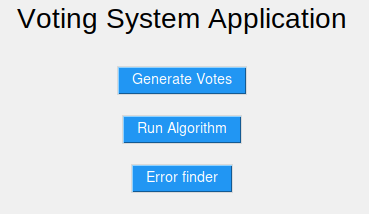
\includegraphics[width=12cm]{user_interface_main.png}
	\end{center}
	
	\section{Generate votes}
	
	If you clicked in the main menu on the generate votes this window pop up:
	
	\begin{center}
		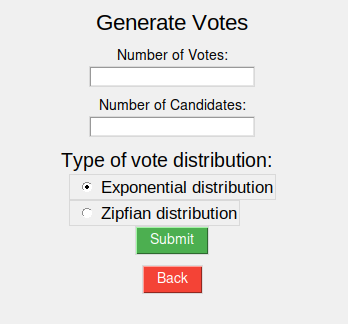
\includegraphics[width=12cm]{generate_votes.png}
	\end{center}
	
	Clicking back will lead you back into main menu. If you put in all the informations and click "Choose files and run"\ the program will ask where it should save the generated vote file. That looks like this.
	
	\begin{center}
		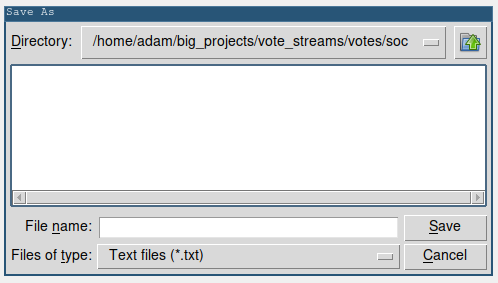
\includegraphics[width=12cm]{save_as.png}
	\end{center}
	
	The file with generated votes will apear there.
	
	\section{Run algorithm}
	
	If you clicked run algorithm this will apear:
	
	\begin{center}
		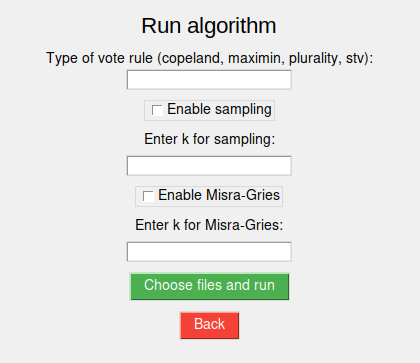
\includegraphics[width=12cm]{run_algorithm.png}
	\end{center}
	
	In the "Type of vote rule"\ you have these options:
	
	\begin{itemize}
		\item STV
		\item Plurality
		\item Minimax
		\item Copeland
	\end{itemize}
	
	The capitalization of the letters in that doesnt metter. Then you choose if you want to have enabled sampling or Misra Gries and put there the $k$ for tham. In sampling $k$ is that every $k$-th vote will be choosen, for $k = 3$ it will be number of votes // $k$. In Misra Gries it is the classical parametr of Misra Gries algorithm. Make sure you dont choose both sampling and Misra Gries at the same time, then the program wont let you further. Then you click "Choose files and run"\ same dialog as in Generate votes will appear for choosing the files, except now you can choose more files as an input. And then save file same as before. And the program will generate the winners.
	
	\section{Error finder}
	
	If clicked the Error finder the only thing that will apear is this:
	
	\begin{center}
		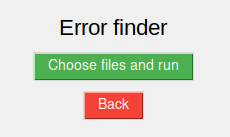
\includegraphics[width=12cm]{error_finder.png}
	\end{center}
	
	Again just click "Choose files and run"\ and the program will ask you to put in the $2$ files and $1$ save file, choose them and the rpogram will find the error between them.
	
	\chapter{Command line interface}
	
	When run with wrong number of arguments the program will output the help messege which is:
	
	\begin{lstlisting}
-g/generate
-- Generate votes with given distribution and save them in file you choose.

-r/run
-- Run algorithm to determinate winner from some votes saved in vote file.

-e/error
-- Find what is error in some aproximated votes, that is you give it twofiles and it find out by some metric how far they are from each other.

-gi/graphical
-- Start graphical interface

-h/help
-- Print larger help messege.
	\end{lstlisting}
	
	It basicly works the same as Graphical interface but when -r is used than just one parametr of $k$ is set, thats because we know that not both sampling and Misra Gries can be used so we use just one. Also when -r is used also one vote file can be given (then you can run it again on different file). If you give it just the argument (like "-e/error") another help messege will pop up with new help that guides you thru (in this example) -e arguments. Like this:
	
	\begin{itemize}
		\item -g/generate [save\_path] [num\_votes] [num\_candidates] [generate\_distribution].
		\item -r/run [load\_path] [save\_path] [vote\_type] [sampling\_enable] [misra\_enable] [k]
		\begin{itemize}
			\item for the [sampling\_enable] [misra\_enable] write 1 for true and 0 for false.
			\item k is used for either divide the number of votes when sampling for example k = 2 is "half of the votes"\ or for misra gries as a parametr.
			\item Optionaly the [sampling\_enable] [misra\_enable] [k] can be ignored if you dont plan using them.
		\end{itemize}
		\item -e/error [load\_path1] [load\_path2] [save\_path]
		\begin{itemize}
			\item\ [load\_path1] is the pathe that will be transformed into [load\_path2].
		\end{itemize}
	\end{itemize}
	
	
\end{document}